
    %%%%% %%%%% %%%%%
    %               %
    % New row       %
    %               %
    %%%%% %%%%% %%%%%
\begin{columns}[t]
  \begin{column}{0.40\textwidth}
    \begin{block}{\large Depth and heterozygosity}
%\small

      \begin{columns}
        \begin{column}{0.45\textwidth}
          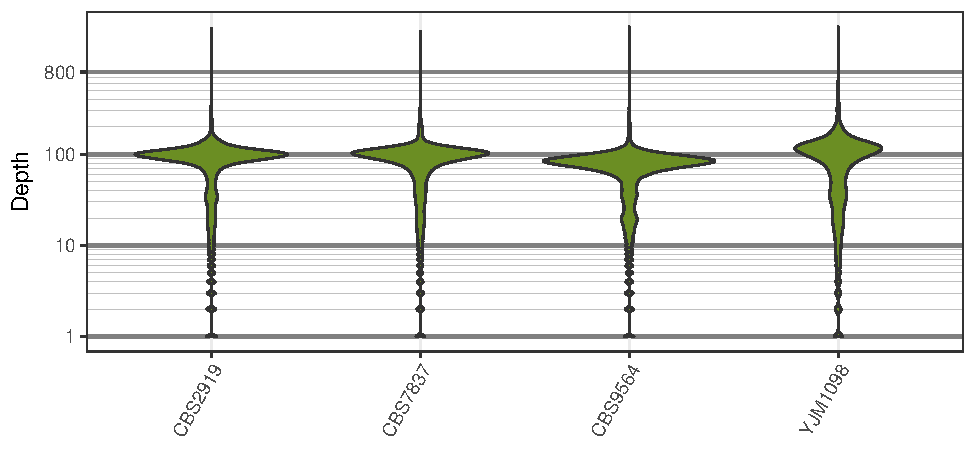
\includegraphics[height=8cm]{./figures/fig2_scer_dp_vplot.pdf}
          \newline
          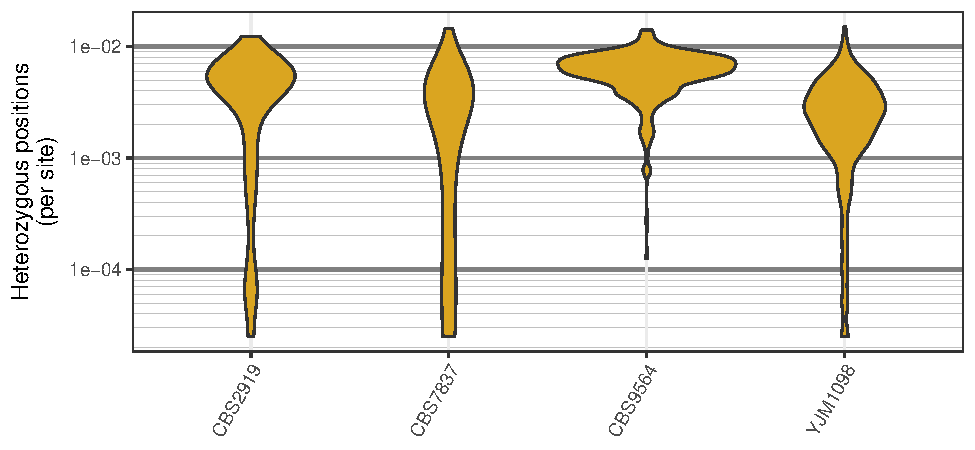
\includegraphics[height=8cm]{./figures/fig3_scer_het_vplot.pdf}
        \end{column}
        \begin{column}{0.53\textwidth}
%\footnotesize
\scriptsize
\\
\vspace{10mm}
Here we summarize the per window sequencing depth and rate of heterozygosity throughhout \textit{S. cerevisiae} genomes.
This can be used to identify regions of the genome that are anomalous.
For example, we observe long tails of low heterozygosity that may be regions of lost heterozygosity.
\vspace{22mm}
        \end{column}
      \end{columns}

    \end{block}
  \end{column}

  \begin{column}{0.52\textwidth}
    \begin{block}{\large Allele balance}
      \begin{columns}
        \begin{column}{0.49\textwidth}
%\small
%\footnotesize
\scriptsize
%\tiny
\\
\vspace{1mm}
Allele balance is the frequency that the most abundant and second most abundant allele were sequenced at.
For diploids we expect half of the sequences to be from each allele.
For triploids we expect the alleles to be sequenced at frequencies of one thirds (1/3 and 2/3).
For tetraploids we expect the alleles to be sequenced at frequencies of quarters (1/4, 1/2, and 3/4).
This information can be used to assign a copy number to a genome or a genomic fraction.
%\vspace{20mm}
%          \begin{figure}
        \end{column}
        \begin{column}{0.4\textwidth}
          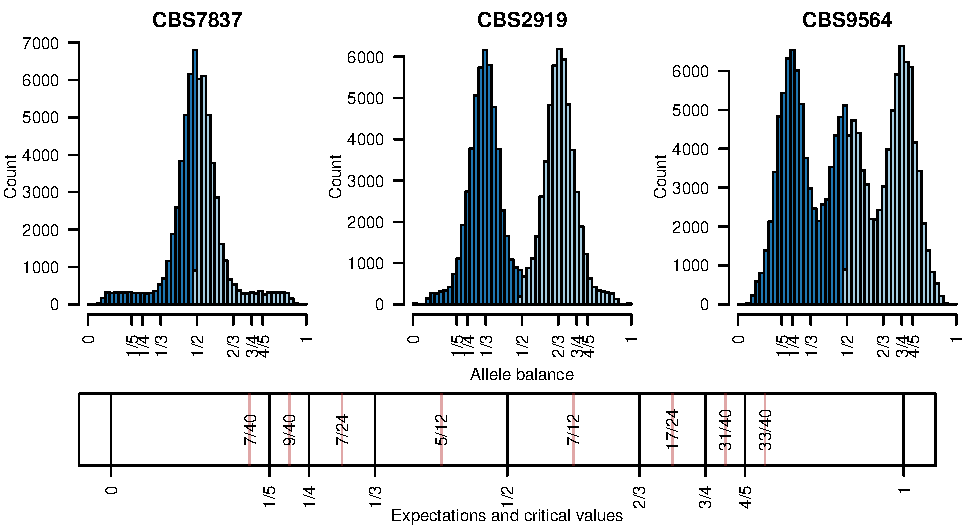
\includegraphics[height=14cm]{./figures/fig1_ab_example.pdf}
        \end{column}
      \end{columns}
%          \caption{Allele balance is the frequency theat the most abundant and second most abundant allele were sequenced at.}
%          \end{figure}

    \end{block}
  \end{column}


\end{columns}


